\let\negmedspace\undefined
\let\negthickspace\undefined
\documentclass[journal,12pt,onecolumn]{IEEEtran}
\usepackage{gvv-book}
\usepackage{gvv}
\usepackage{mathtools}
\usepackage{amssymb,amsfonts,amsthm}
\usepackage{siunitx}
\usepackage{algorithmic}
\usepackage{graphicx}
\graphicspath{{./figs/}}
\usepackage{textcomp}
\usepackage{xcolor}
\usepackage{txfonts}
\usepackage{listings}
\usepackage{enumitem}
\usepackage{gensymb}
\usepackage{comment}
\usepackage{caption}
\usepackage{tkz-euclide}
\usepackage[latin1]{inputenc}
\usepackage{color}
\usepackage{array}
\usepackage{longtable}
\usepackage{calc}
\usepackage{multirow}
\usepackage{multicol}
\usepackage{hhline}
\usepackage{ifthen}
\usepackage{lscape}
\usepackage{tabularx}
\usepackage{float}
\usepackage[breaklinks=true]{hyperref}
\usepackage{cite}

\begin{document}


\begin{center}
\large\textbf{GATE 2019 General aptitude}
\end{center}

\vspace{2em}

\textbf{Q.1 -Q.5 carry one mark each}

\begin{enumerate}[itemsep=0.5cm]
    
\item The fishermen, \underline{\hspace{2cm}}  the flood victims owed their lives, were rewarded by the government.

\hfill{\brak{\text{GATE IN 2019}}}
\begin{multicols}{4}
\begin{enumerate}
    \item whom
    \item to which
    \item to whom
    \item that
\end{enumerate}
\end{multicols}

\item Some students were not involved in the strike.\\
If the above statement is true, which of the following conclusions is/are logically necessary?

\vspace{1em}

    1. Some who were involved in the strike were students.\\
    2. No student was involved in the strike.\\
    3. At least one student was involved in the strike.\\
    4. Some who were not involved in the strike were students.

\hfill{\brak{\text{GATE IN 2019}}}    

\begin{multicols}{4}
\begin{enumerate}
    \item 1 and 2
    \item 3
    \item 4
    \item 2 and 3
\end{enumerate}
\end{multicols}

\item The radius as well as the height of a circular cone increases by 10\%. The percentage increase in its volume is

\hfill{\brak{\text{GATE IN 2019}}}

\begin{multicols}{4}
\begin{enumerate}
    \item 17.1
    \item 21.0
    \item 33.1
    \item 72.8
\end{enumerate}
\end{multicols}

\item Five numbers 10, 7, 5, 4 and 2 are to be arranged in a sequence from left to right following the directions given below:\\

\vspace{1em}

1. No two odd or even numbers are next to each other.\\
2. The second number from the left is exactly half of the left-most number.\\
3. The middle number is exactly twice the right-most number.\\
Which is the second number from the right?

\hfill{\brak{\text{GATE IN 2019}}}

\begin{multicols}{2}
\begin{enumerate}
    \item 2
    \item 4
    \item 7
    \item 10
\end{enumerate}
\end{multicols}

\item Until Iran came along, India had never been in kabaddi.

\hfill{\brak{\text{GATE IN 2019}}}

\begin{multicols}{4}
\begin{enumerate}
    \item defeated
    \item defeating
    \item defeat
    \item defeatist
\end{enumerate}
\end{multicols}

\newpage

\textbf{Q.6 -Q.10 carry two marks each}

\vspace{2em}

\item Since the last one year, after a 125 basis point reduction in repo rate by the Reserve Bank of India, banking institutions have been making a demand to reduce interest rates on small saving schemes. Finally, the government announced yesterday a reduction in interest rates on small saving schemes to bring them on par with fixed deposit interest rates.

\vspace{1em}

Which one of the following statements can be inferred from the given passage?

\hfill{\brak{\text{GATE IN 2019}}}


\begin{enumerate}
    \item Whenever the Reserve Bank of India reduces the repo rate, the interest rates on small saving schemes are also reduced
    \item Interest rates on small saving schemes are always maintained on par with fixed deposit interest rates
    \item The government sometimes takes into consideration the demands of banking institutions before reducing the interest rates on small saving schemes
    \item A reduction in interest rates on small saving schemes follow only after a reduction in repo rate by the Reserve Bank of India
\end{enumerate}

\vspace{2em}


\item In a country of 1400 million population, 70\% own mobile phones. Among the mobile phone owners, only 294 million access the Internet. Among these Internet users, only half buy goods from e-commerce portals. What is the percentage of these buyers in the country?

\hfill{\brak{\text{GATE IN 2019}}}

\begin{multicols}{4}
\begin{enumerate}
    \item 10.50
    \item 14.70
    \item 15.00
    \item 50.00
\end{enumerate}
\end{multicols}

\vspace{1em}

\item The nomenclature of Hindustani music has changed over the centuries. Since the medieval period \textit{dhrupad} styles were identified as \textit{bauntis}. Terms like \textit{gayaki} and \textit{baaj} were used to refer to vocal and instrumental styles, respectively. With the institutionalization of music education the term \textit{gharana} became acceptable. \textit{Gharana} originally referred to hereditary musicians from a particular lineage, including disciples and grand disciples.

Which one of the following pairings is NOT correct?

\hfill{\brak{\text{GATE IN 2019}}}


\begin{enumerate}
    \item \textit{dhrupad}, \textit{baant}
    \item \textit{gayaki}, vocal
    \item \textit{baaj}, institution
    \item \textit{gharana}, lineage
\end{enumerate}

\vspace{1em}

\item Two trains started at 7\,AM from the same point. The first train travelled north at a speed of 80\,km/h and the second train travelled south at a speed of 100\,km/h. The time at which they were 540\,km apart is AM.

\hfill{\brak{\text{GATE IN 2019}}}

\begin{multicols}{4}
\begin{enumerate}
    \item 9
    \item 10
    \item 11
    \item 11.30
\end{enumerate}
\end{multicols}


\item "I read somewhere that in ancient times the prestige of a kingdom depended upon the number of taxes that it was able to levy on its people. It was very much like the prestige of a head-hunter in his own community."

\vspace{2em}

Based upon the paragraph above, the prestige of a head-hunter depended upon, 

\hfill{\brak{\text{GATE IN 2019}}}

\begin{enumerate}
    \item the prestige of the kingdom
    \item the prestige of the heads
    \item the number of taxes he could levy
    \item the number of heads he could gather
\end{enumerate}


\vspace{5em}


\begin{center}
    \large\textbf{END OF THE QUESTION PAPER}
\end{center}

\end{enumerate}

\newpage

\textbf{Q.1 -Q.5 carry one mark each}

\vspace{2em}

\begin{enumerate}[itemsep=0.45cm]
\item The relative magnetic permeability of a type-I superconductor is

\hfill{\brak{\text{GATE IN 2019}}}

\begin{multicols}{4}
\begin{enumerate}
    \item $0$
    \item $-1$
    \item $2\pi$
    \item $\dfrac{1}{4\pi}$
\end{enumerate}
\end{multicols}

\item Considering baryon number and lepton number conservation laws, which of the following processes is/are allowed?
\[
(1)\quad p \rightarrow \pi^{0} + e^{+} + \nu_{e}
\qquad\qquad
(2)\quad e^{+} + \nu_{e} \rightarrow \mu^{+} + \nu_{\mu}
\]

\hfill{\brak{\text{GATE IN 2019}}}

\begin{multicols}{2}
\begin{enumerate}
    \item both (1) and (2)
    \item only (1)
    \item only (2)
    \item neither (1) nor (2)
\end{enumerate}
\end{multicols}

\item For the following circuit, what is the magnitude of $V_{\text{out}}$ if $V_{\text{in}}=1.5\ \mathrm{V}$?

\hfill{\brak{\text{GATE IN 2019}}}

\begin{figure}[ht!]
    \centering
    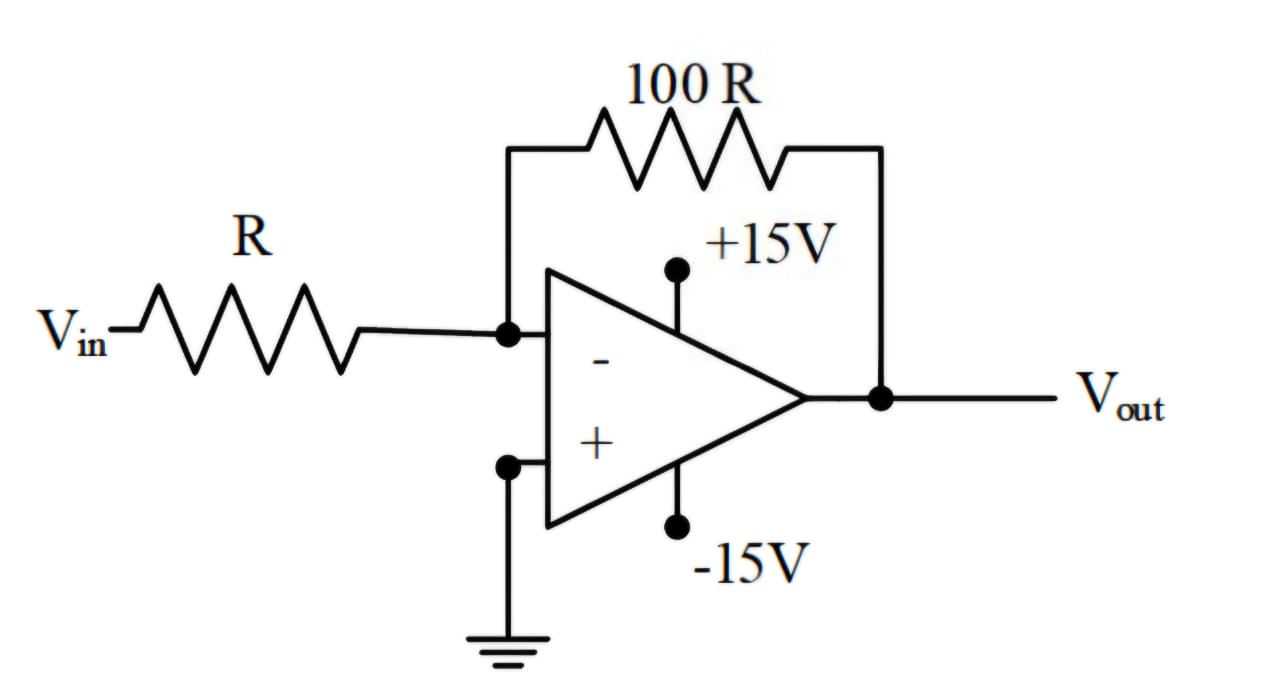
\includegraphics[width=0.75\textwidth]{fig1.jpeg}
    \caption{}
    \label{fig:fig1.jpeg}
\end{figure}

\begin{multicols}{2}
\begin{enumerate}
    \item $0.015\ \mathrm{V}$
    \item $0.15\ \mathrm{V}$
    \item $15\ \mathrm{V}$
    \item $150\ \mathrm{V}$
\end{enumerate}
\end{multicols}

\item For the differential equation (where $n$ is a constant), the product of its two independent solutions is

\hfill{\brak{\text{GATE IN 2019}}}
\begin{multicols}{4}
\begin{enumerate}
    \item $\dfrac{1}{x}$
    \item $x$
    \item $x^{n}$
    \item $\dfrac{1}{x^{\,n+1}}$
\end{enumerate}
\end{multicols}

\newpage

\item Consider a one-dimensional gas of $N$ non-interacting particles of mass $m$ with the Hamiltonian for a single particle given by
\[
H = \frac{p^2}{2m} + \frac{1}{2} m a s^2 (x^2 + 2x)
\]
The high temperature specific heat in units of $R = N k_B$ (where $k_B$ is the Boltzmann constant) is

\hfill{\brak{\text{GATE IN 2019}}}


\begin{enumerate}
\item 1
\item 1.5
\item 2
\item 2.5
\end{enumerate}

\item An electric field $E = E_0 z^2$ is applied to a Hydrogen atom in the $n=2$ excited state. Ignoring spin, the $\alpha = 2$ fourfold degenerate states in the $|n,l,m\rangle$ basis are given by $|0,0\rangle$, $|1,1\rangle$, $|1,0\rangle$, and $|1,-1\rangle$. If $H'$ is the interaction Hamiltonian corresponding to the applied electric field, which of the following matrix elements is nonzero?

\hfill{\brak{\text{GATE IN 2019}}}


\begin{enumerate}
\item $\langle 0,0| H' |1,0\rangle$
\item $\langle 0,0| H' |1,1\rangle$
\item $\langle 0,0| H' |1,-1\rangle$
\item $\langle 0,0| H' |1,0\rangle$
\end{enumerate}


\item A large number $N$ of ideal bosons, each of mass $m$, are trapped in a three-dimensional potential $V(r) = \frac{1}{2} m \omega^2 r^2$. The bosonic system is kept at temperature $T \ll T_c$ (much lower than the Bose-Einstein condensation temperature $T_c$). The chemical potential $\mu$ satisfies

\hfill{\brak{\text{GATE IN 2019}}}


\begin{enumerate}
\item $\mu \le \frac{3}{2} \hbar \omega$
\item $2\hbar\omega > \mu > \frac{3}{2} \hbar \omega$
\item $3\hbar\omega > \mu > 2 \hbar \omega$
\item $\mu = 0$
\end{enumerate}


\item During a rotation, vectors along the axis of rotation remain unchanged. For the rotation matrix, the unit vector along the axis of rotation is
\[
\myvec{0 & 1 & 0 \\ 0 & 0 & -1 \\ -1 & 0 & 0}
\]

\hfill{\brak{\text{GATE IN 2019}}}

\begin{multicols}{4}
\begin{enumerate}
\item $\frac{1}{3} (2 \hat{i} - \hat{j} + 2 \hat{k})$
\item $\frac{1}{\sqrt{3}} (\hat{i} + \hat{j} - \hat{k})$
\item $\frac{1}{\sqrt{3}} (\hat{i} - \hat{j} - \hat{k})$
\item $\frac{1}{3} (2 \hat{i} + 2 \hat{j} - \hat{k})$
\end{enumerate}
\end{multicols}


\item For a spin-$\frac{1}{2}$ particle, let $|\uparrow\rangle$ and $|\downarrow\rangle$ denote its spin-up and spin-down states, respectively.  
\[
|a\rangle = \frac{1}{\sqrt{2}} \big(|\uparrow\rangle|\downarrow\rangle + |\downarrow\rangle|\uparrow\rangle \big), \quad
|b\rangle = \frac{1}{\sqrt{2}} \big(|\uparrow\rangle|\downarrow\rangle - |\uparrow\rangle|\downarrow\rangle \big)
\]  
are composite states of the following total spin $S$:

\hfill{\brak{\text{GATE IN 2019}}}


\begin{enumerate}
\item $S = 1$ for $a$, and $b$ is not an eigenstate of the operator $\tilde{S}^2$
\item not an eigenstate of the operator $\tilde{S}^2$ and $S=0$ for $b$
\item $S=0$ for $a$, and $S=1$ for $b$
\item $S=1$ for $a$, and $S=0$ for $b$
\end{enumerate}


\item Consider a transformation from one set of generalized coordinates and momenta $(q,p)$ to another set $(Q,P)$ denoted by
\begin{align*}    
Q = p q^k \quad 
P = \mathfrak{q}^r:
\end{align*}

\text{where $s$ and $r$ are constants.}

The transformation is canonical if 

\hfill{\brak{\text{GATE IN 2019}}}


\begin{multicols}{4}
\begin{enumerate}
\item $s = ?$ and $r = 1, s=0$
\item $s = 2$ and $r = -1$
\item $s = 0, r = -1$
\item $s = 2, r = 1$
\end{enumerate}
\end{multicols}

\item In order to estimate the specific heat of phonons, the appropriate method to apply would be:

\hfill{\brak{\text{GATE IN 2019}}}

\begin{enumerate}
\item Einstein model for acoustic phonons and Debye model for optical phonons
\item Einstein model for optical phonons and Debye model for acoustic phonons
\item Einstein model for both optical and acoustic phonons
\item Debye model for both optical and acoustic phonons
\end{enumerate}


\item The pole of the function $f(z)\cot z$ at $z = 0$ is:

\hfill{\brak{\text{GATE IN 2019}}}

\begin{multicols}{2}
\begin{enumerate}
\item a removable singularity
\item an essential singularity
\item a simple pole
\item a second order pole
\end{enumerate}
\end{multicols}

\item A massive particle $X$ in free space decays spontaneously into two photons. Which of the following statements is true for $X$?

\hfill{\brak{\text{GATE IN 2019}}}


\begin{enumerate}
\item $X$ is charged
\item Spin of $X$ must be greater than or equal to 2
\item $X$ is a boson
\item $X$ must be a baryon
\end{enumerate}


\item The electric field of an electromagnetic wave is given by
\[
\vec{E} = 3 \sin(kx - \alpha t) \hat{x} + 4 \cos(kz - \omega t) \hat{y}
\]  
The wave is

\hfill{\brak{\text{GATE IN 2019}}}



\begin{enumerate}
\item linearly polarized at an angle $\arctan(4/3)$ from the x-axis
\item linearly polarized at an angle $\arctan(3/4)$ from the x-axis
\item elliptically polarized in clockwise direction when seen travelling towards the observer
\item elliptically polarized in counter-clockwise direction when seen travelling towards the observer
\end{enumerate}


\item The nuclear spin and parity of Ca in its ground state is

\hfill{\brak{\text{GATE IN 2019}}}

\begin{multicols}{4}
\begin{enumerate}
\item 0
\item 0
\item 1
\item 1
\end{enumerate}
\end{multicols}

\item An infinitely long thin cylindrical shell has its axis coinciding with the $z$-axis. It carries a surface charge density $\sigma = \sigma_0 \cos\phi$, where $\phi$ is the polar angle and $\sigma_0$ is a constant.  
The magnitude of the electric field *inside* the cylinder is

\hfill{\brak{\text{GATE IN 2019}}}

\begin{multicols}{4}
\begin{enumerate}
\item $0$
\item $\sigma_0/(2\epsilon_0)$
\item $\sigma_0/(3\epsilon_0)$
\item $\sigma_0/(4\epsilon_0)$
\end{enumerate}
\end{multicols}

\item Consider a three-dimensional crystal of $N$ inert gas atoms. The total energy is
\[
U(R) = 2 N c \big[ p (\sigma/R)^{12} - q (\sigma/R)^6 \big]
\]  
where $p = 12.13$, $q = 14.45$, and $R$ is the nearest neighbour separation. The constants $\epsilon$ and $\sigma$ have dimensions of energy and length, respectively.  
The *equilibrium separation* between two nearest neighbour atoms (in units of $\sigma$, rounded to two decimal places) is \dots

\hfill{\brak{\text{GATE IN 2019}}}

\item The energy-wavevector ($E-k$) dispersion relation for a particle in two dimensions is
\[
E = C k
\]  
where $C$ is a constant. If the density of states $D(E) \propto E^p$, the value of $p$ is \dots

\hfill{\brak{\text{GATE IN 2019}}}

\item A circular loop made of thin wire has radius $2\,\mathrm{cm}$ and resistance $2\,\Omega$. It is placed perpendicular to a uniform magnetic field of magnitude $|\vec{B}_0| = 0.01\,\mathrm{T}$. At $t=0$, the field starts decaying as
\[
\vec{B} = \vec{B}_0 e^{-t/t_0}, \quad t_0 = 1\,\mathrm{s}
\]  
The total charge that passes through a cross section of the wire during the decay is $Q$. The value of $Q$ in $\mu\mathrm{C}$ (rounded off to two decimal places) is \dots

\hfill{\brak{\text{GATE IN 2019}}}

\newpage



\item The electric field of an electromagnetic wave in vacuum is given by
\[
\vec{E} = E_0 \cos(3y + 4z - 1.5 \times 10^9 t)
\]  
The wave is reflected from the surface. If the pressure exerted on the surface is $E_g$, the value of $\alpha$ (rounded to one decimal place) is \dots

\hfill{\brak{\text{GATE IN 2019}}}


\item The Hamiltonian for a quantum harmonic oscillator of mass $m$ in three dimensions is
\[
H = \frac{\vec{p}^{\,2}}{2m} + \frac{1}{2} m \omega^2 r^2
\]  
where $\omega$ is the angular frequency. The expectation value of $r^2$ in the first excited state of the oscillator (in units of $\hbar / m\omega$, rounded to one decimal place) is \dots

\hfill{\brak{\text{GATE IN 2019}}}

\item The Hamiltonian for a particle of mass $m$ is
\[
H = \frac{p^2}{2m}
\]  
where $q$ and $p$ are the generalized coordinate and momentum, respectively; $t$ is time and $k$ is a constant. For the initial condition $q = 0$ and $p = 0$ at $t = 0$, $q(t) = ?$. The value of $\alpha$ is \dots

\hfill{\brak{\text{GATE IN 2019}}}

\item At temperature $T$ Kelvin (K), the value of the Fermi function at an energy $0.5\,\mathrm{eV}$ above the Fermi energy is $0.01$. Then $\beta$, to the nearest integer, is \dots  
($k_B = 8.62 \times 10^{-5}\,\mathrm{eV/K}$)

\hfill{\brak{\text{GATE IN 2019}}}

\item Let 
\begin{align}
\psi_1\rangle = \myvec{1 \\ 0} \\
\psi_2\rangle = \myvec{0 \\ 1}
\end{align}

represent two possible states of a two-level quantum system. The state obtained by the incoherent superposition of $|\psi_1\rangle$ and $|\psi_2\rangle$ is given by the density matrix
\[
\rho = c_1 |\psi_1\rangle \langle \psi_1| + c_2 |\psi_2\rangle \langle \psi_2|
\]  
If $c_1 = 0.4$ and $c_2 = 0.6$, the matrix element $P_{22}$ (rounded off to one decimal place) is \dots

\hfill{\brak{\text{GATE IN 2019}}}

\item A conventional type-I superconductor has a critical temperature of $4.7\,\mathrm{K}$ at zero magnetic field and a critical magnetic field of $0.3\,\mathrm{T}$ at $0\,\mathrm{K}$. The critical field in Tesla at $2\,\mathrm{K}$ (rounded off to three decimal places) is \dots

\hfill{\brak{\text{GATE IN 2019}}}


\newpage

\item Consider the following Boolean expression:
    \[
    (\overline{A} + \overline{B})[\overline{A}(B + C)] + A(\overline{B} + \overline{C})
    \]
    It can be represented by a single three-input logic gate. Identify the gate.

\hfill{\brak{\text{GATE IN 2019}}}


    \begin{multicols}{4}
    \begin{enumerate}
        \item AND
        \item OR
        \item XOR
        \item NAND
    \end{enumerate}
    \end{multicols}

\item The value of the integral 
    \[
    \int_{-\infty}^{\infty} \frac{\cos(kx)}{x^2 + a^2} \, dx, \quad k>0, \, a>0
    \]

\hfill{\brak{\text{GATE IN 2019}}}


    \begin{multicols}{4}
    \begin{enumerate}
        \item $\frac{\pi}{a} e^{-ka}$
        \item $\frac{2\pi}{a} e^{-ka}$
        \item $\frac{\pi}{2a} e^{-ka}$
        \item $\frac{3\pi}{2a} e^{-ka}$
    \end{enumerate}
    \end{multicols}

\item The wave function $\psi(x)$ of a particle is as shown below. Here $K$ is a constant, and $a>d$. The position uncertainty $(\Delta x)$ of the particle is

\begin{figure}[ht!]
    \centering
    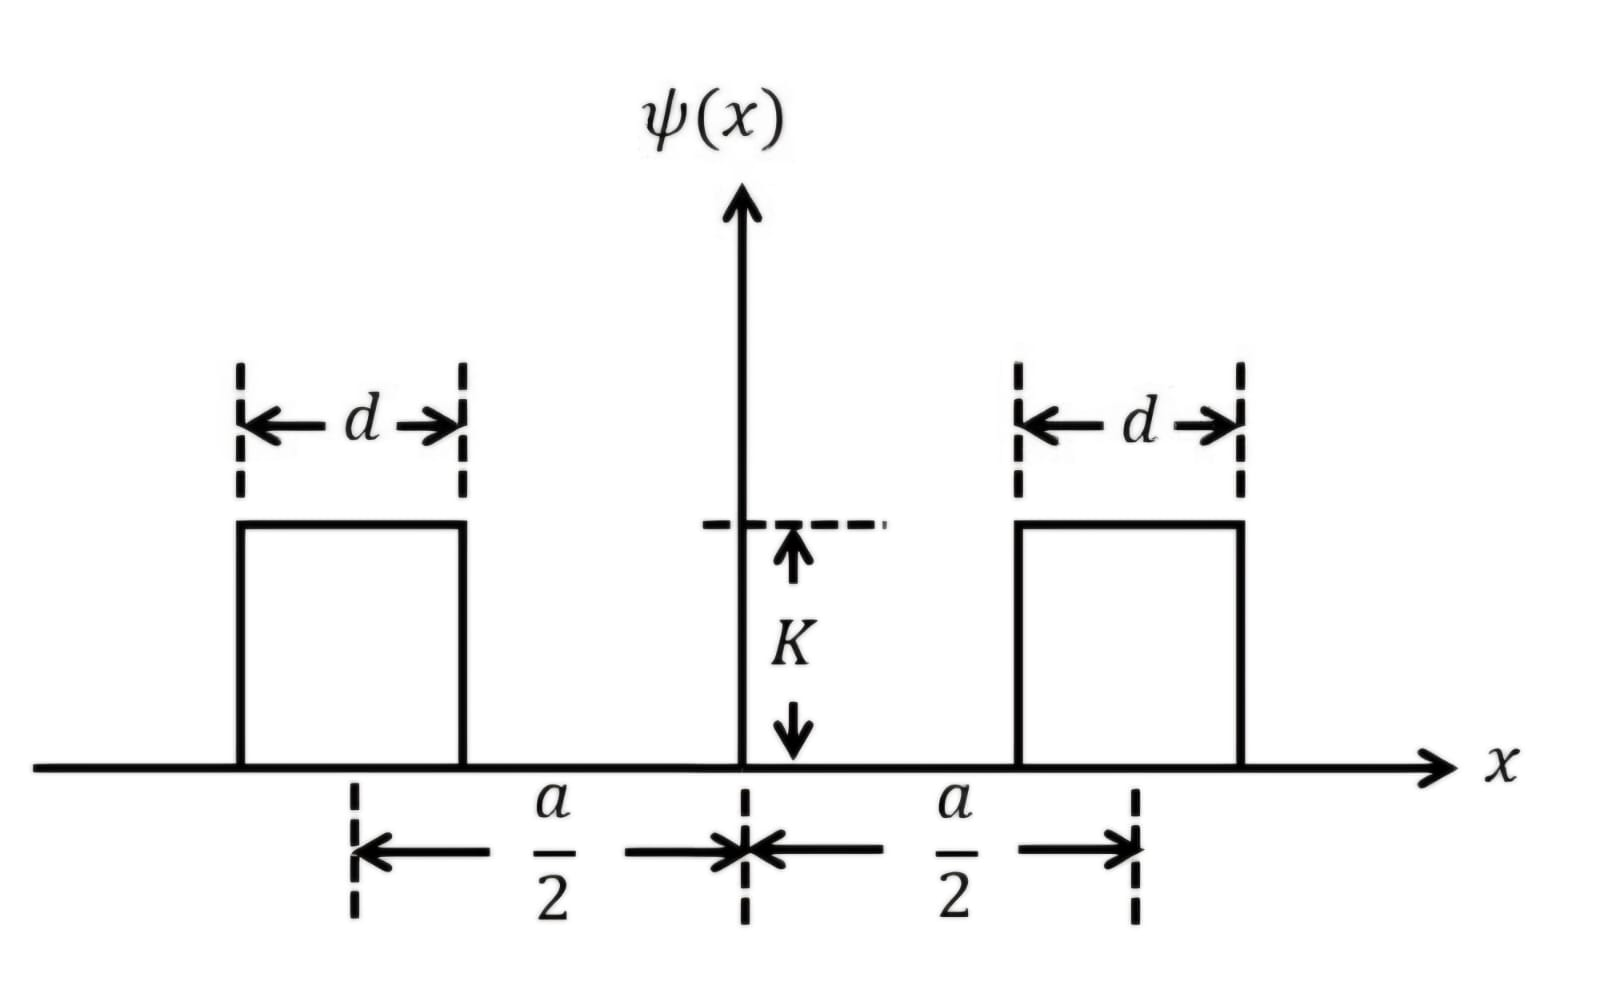
\includegraphics[width=0.75\textwidth]{fig2.jpeg}
    \caption{}
    \label{fig:fig2.jpeg}
\end{figure}


\hfill{\brak{\text{GATE IN 2019}}}

    \begin{multicols}{4}
    \begin{enumerate}
        \item $\sqrt{\frac{a^2 + 3d^2}{12}}$
        \item $3\sqrt{\frac{3a^2 + d^2}{12}}$
        \item $\sqrt{\frac{d^2}{6}}$
        \item $\sqrt{\frac{d^2}{34}}$
    \end{enumerate}
    \end{multicols}

\item A solid cylinder of radius $R$ has total charge $Q$ distributed uniformly over its volume. It is rotating about its axis with angular speed $\omega$. The magnitude of the total magnetic moment of the cylinder is

\hfill{\brak{\text{GATE IN 2019}}}


    \begin{multicols}{2}
    \begin{enumerate}
        \item $Q R^2 \omega$
        \item $Q R \omega$
        \item $Q R w$
        \item $-Q R w$
    \end{enumerate}
    \end{multicols}

\item Consider the motion of a particle along the $x$-axis in a potential $V(x)=Fx$. Its ground state energy $E_g$ is estimated using the uncertainty principle. Then $E_g$ is proportional to

\hfill{\brak{\text{GATE IN 2019}}}

    \begin{multicols}{4}
    \begin{enumerate}
        \item $F^{1/3}$
        \item $F^{1/2}$
        \item $F^{2/5}$
        \item $F^{2/3}$
    \end{enumerate}
    \end{multicols}



 \item A 3-bit analog-to-digital converter is designed to digitize analog signals ranging from $0\,\mathrm{V}$ to $10\,\mathrm{V}$. For this converter, the binary output corresponding to an input of $6\,\mathrm{V}$ is

 \hfill{\brak{\text{GATE IN 2019}}}

    \begin{multicols}{2}
    \begin{enumerate}
        \item 011
        \item 101
        \item 100
        \item 010
    \end{enumerate}
    \end{multicols}

 \item The Hamiltonian operator for a two-level quantum system is
    \[
      H=\myvec{E_1 & 0\\ 0 & E_2}
    \]
    If the state at $t=0$ is
    \[
      \lvert \psi(0)\rangle=\frac{1}{\sqrt{2}} \myvec{1\\1}
    \]
    then $\lvert\langle \psi(0)\vert \psi(t)\rangle\rvert^2$ at time $t$ is

    \hfill{\brak{\text{GATE IN 2019}}}

    \begin{multicols}{2}
    \begin{enumerate}
        \item $\tfrac{1}{2}\bigl(1+e^{-(E_1-E_2)t/h}\bigr)$
        \item $\,\bigl(1-e^{-(E_1-E_2)t/h}\bigr)$
        \item $\,\bigl(1+\cos[(E_1-E_2)t/h]\bigr)$
        \item $\,\bigl(1-\cos[(E_1-E_2)t/h]\bigr)$
    \end{enumerate}
    \end{multicols}

 \item A particle of mass $m$ moves in a lattice along the $x$-axis in a periodic potential $V(x)=V(x+d)$ with periodicity $d$. The corresponding Brillouin zone extends from $k_0$ to $k_a$, with these two $k$-points being equivalent. If a weak force $F$ in the $x$-direction is applied to the particle, it starts a periodic motion with time period $\tau$. Using the equation of motion $\dot{p}=F$ for a particle moving in a band, where $p_\text{crystal}$ is the crystal momentum of the particle, the period $\tau$ is (with $h$ the Planck constant)

 \hfill{\brak{\text{GATE IN 2019}}}

    \begin{multicols}{2}
    \begin{enumerate}
        \item $\sqrt{\dfrac{2md}{F}}$
        \item $2\sqrt{\dfrac{2md}{F}}$
        \item $\dfrac{2h}{Fd}$
        \item $\dfrac{h}{Fd}$
    \end{enumerate}
    \end{multicols}

\newpage

\item Consider a potential barrier V of the form


\begin{figure}[ht!]
    \centering
    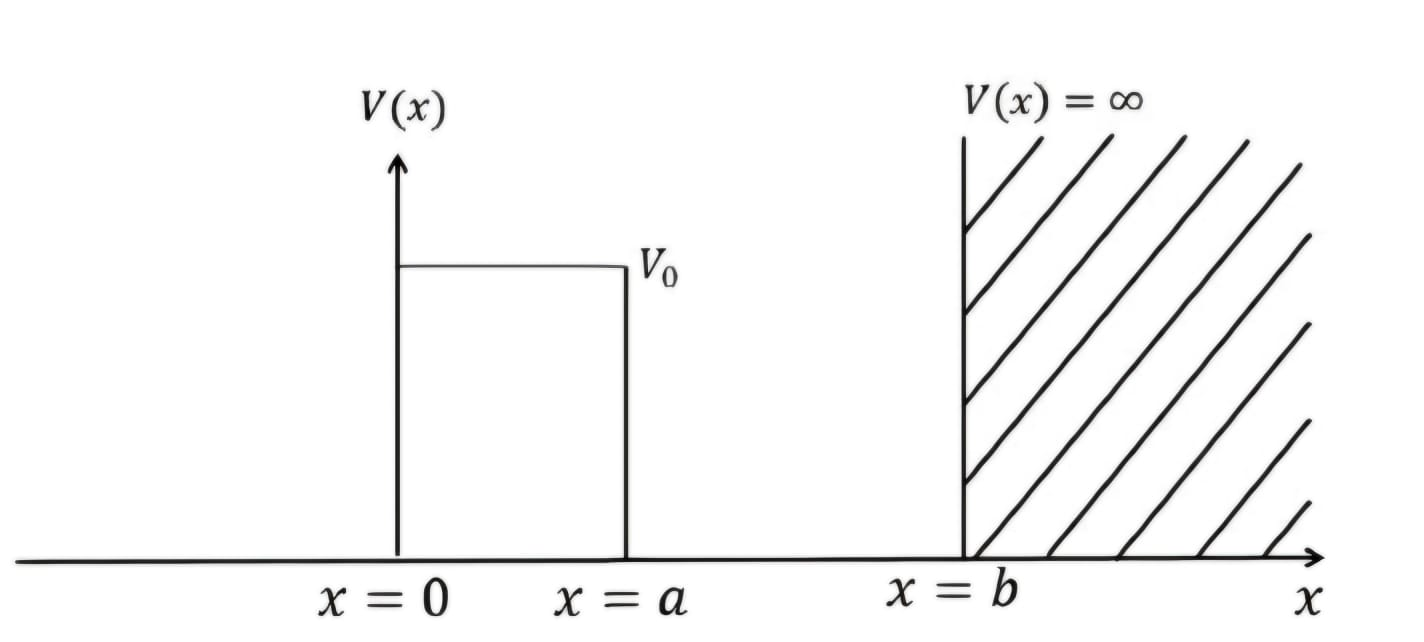
\includegraphics[width=0.75\textwidth]{fig3.jpeg}
    \caption{}
    \label{fig:fig3.jpeg}
\end{figure}

where $V_0$ is a constant. For particles of energy $E<V_0$ incident on this barrier from the left. which of the following schematic diagrams best represent the the probability density as a function of x?

\hfill{\brak{\text{GATE IN 2019}}}

\begin{multicols}{2}
\begin{enumerate}
    \item 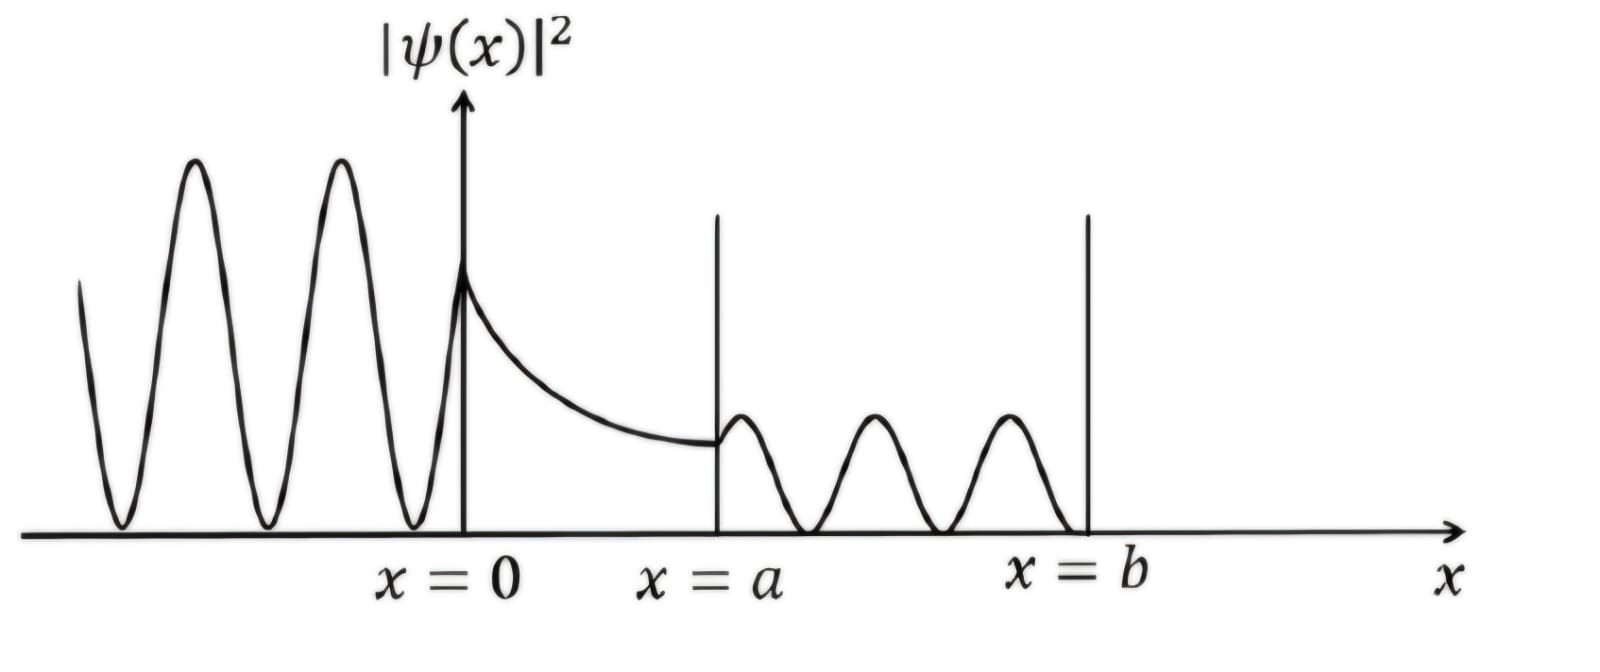
\includegraphics[width=0.35\textwidth]{fig4.jpeg} \hfill
    \item 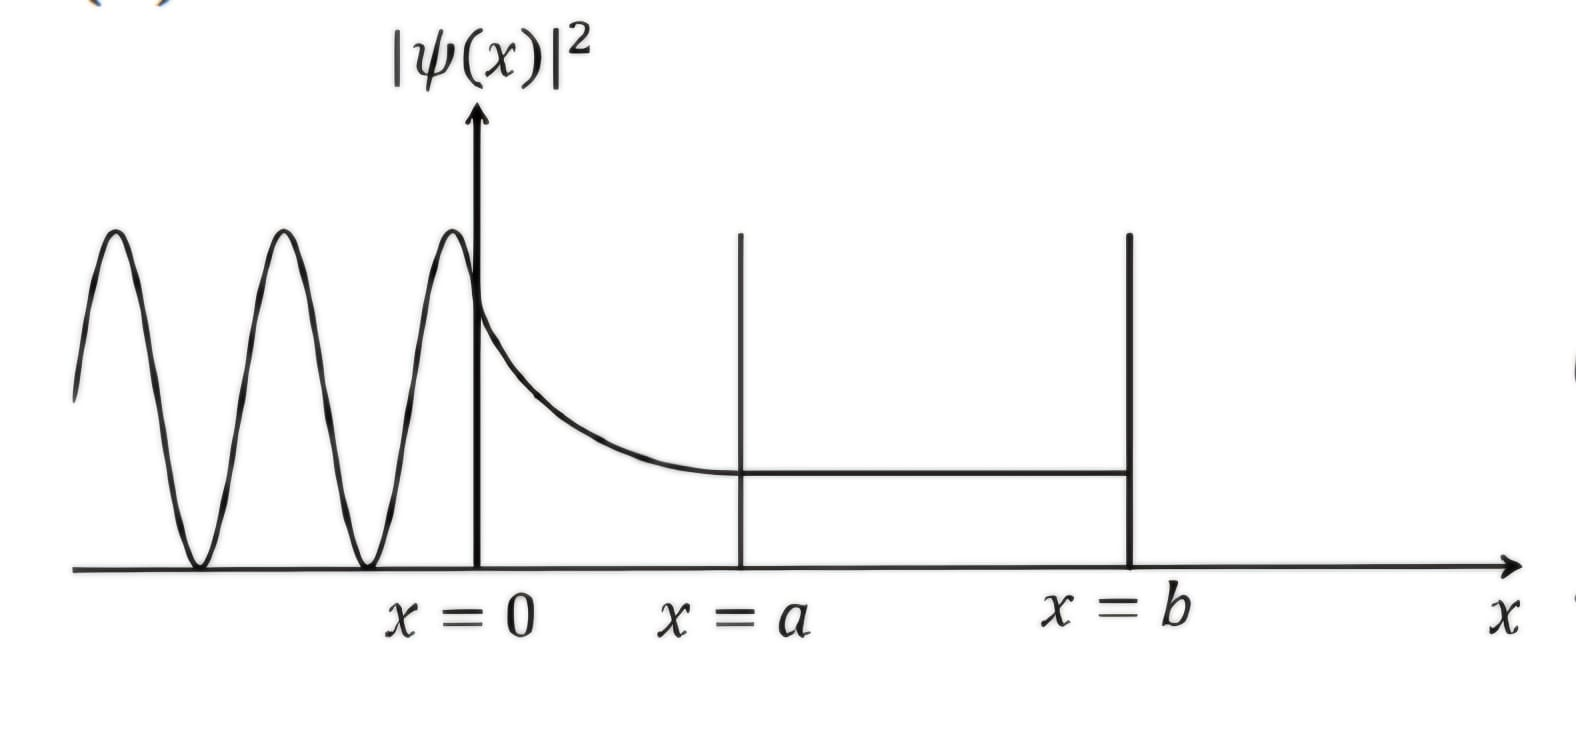
\includegraphics[width=0.35\textwidth]{fig5.jpeg} \hfill
    \item 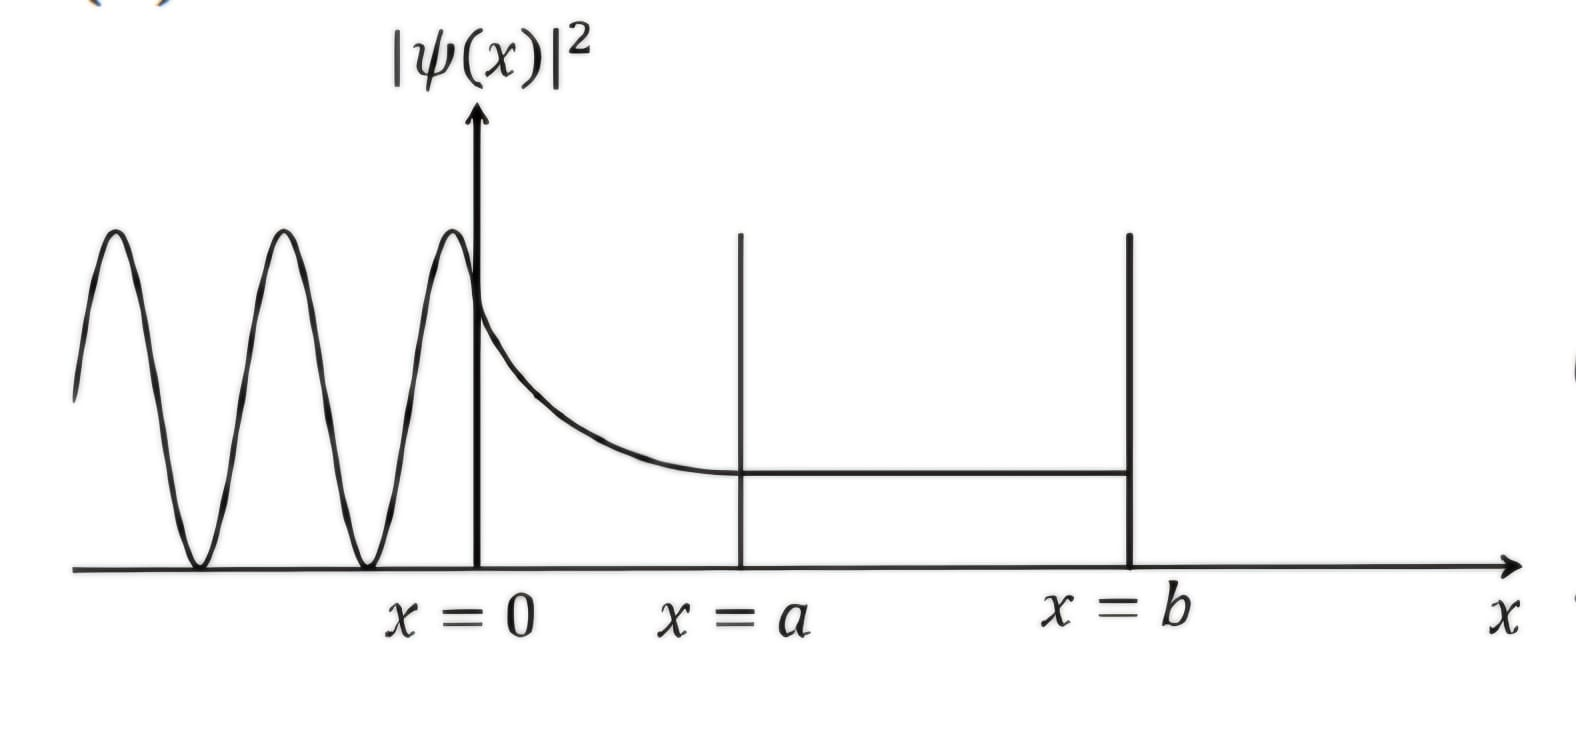
\includegraphics[width=0.35\textwidth]{fig6.jpeg} \hfill
    \item 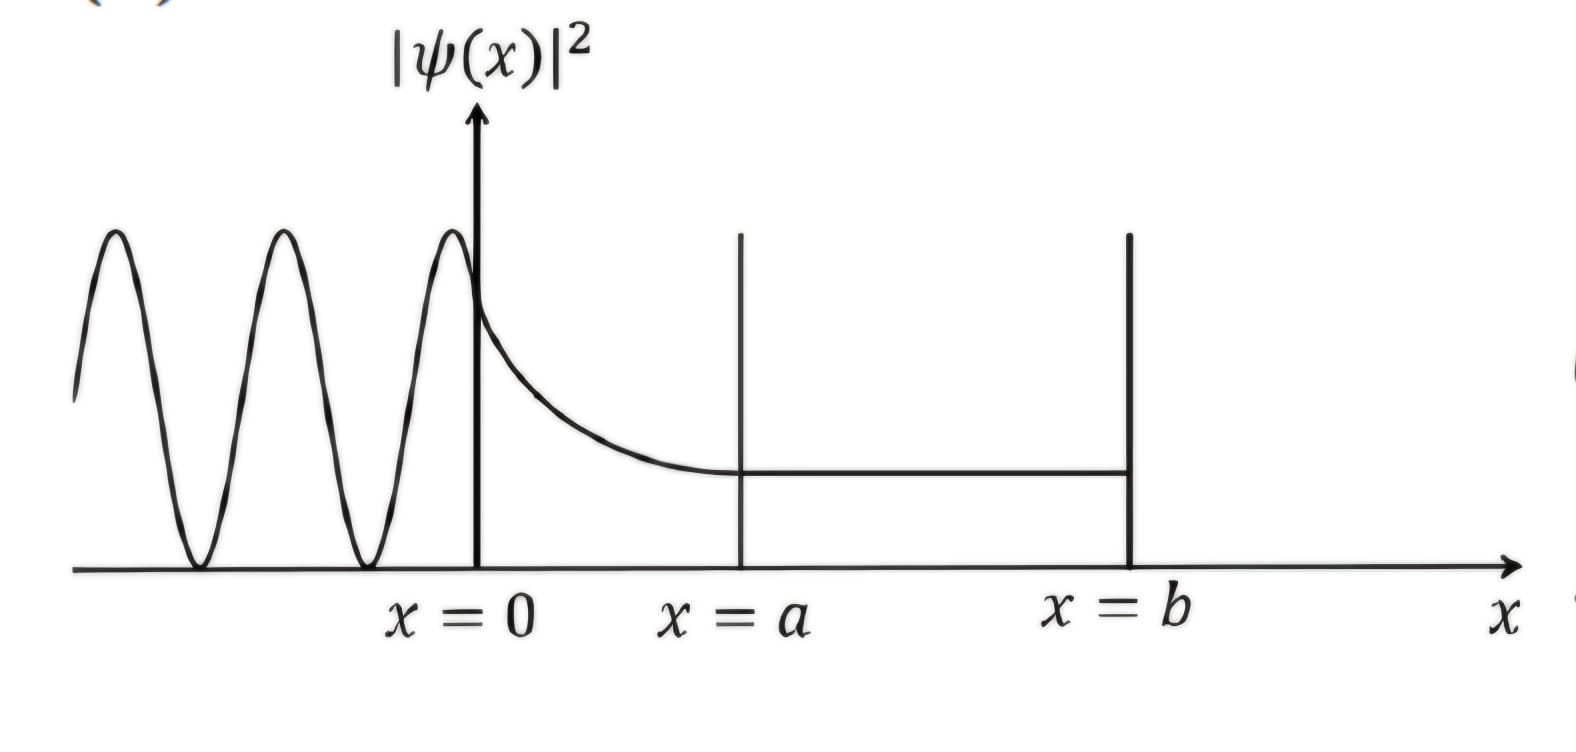
\includegraphics[width=0.35\textwidth]{fig7.jpeg} \hfill
\end{enumerate}
\end{multicols}


\item  In a set of $N$ successive polarizers, the $m^{\text{th}}$ polarizer makes an angle 
    $\dfrac{m\pi}{2N}$ with the vertical. A vertically polarized light beam of intensity $I_{0}$ 
    is incident on two sets with $N=N_{1}$ and $N=N_{2}$, where $N_{2}>N_{1}$. Let the intensities 
    of light beams coming out be $I(N_{1})$ and $I(N_{2})$ respectively. Which of the following 
    statements is correct about the two?

\hfill{\brak{\text{GATE IN 2019}}}
   
    \begin{enumerate}
        \item $I(N_{2}) > I(N_{1})$, the polarization in each case is vertical
        \item $I(N_{2}) < I(N_{1})$, the polarization in each case is vertical
        \item $I(N_{2}) > I(N_{1})$, the polarization in each case is horizontal
        \item $I(N_{2}) < I(N_{1})$, the polarization in each case is horizontal
    \end{enumerate}


\newpage

\item For the following circuit, the correct logic values for the entries X and Y in the truth table are

\begin{figure}[ht!]
    \centering
    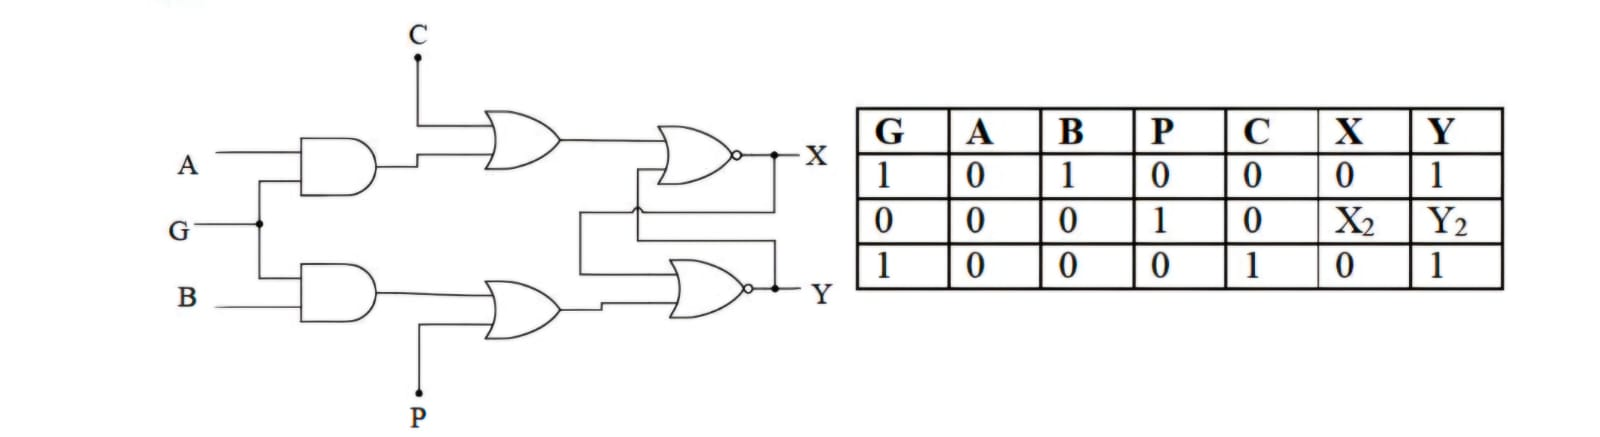
\includegraphics[width=1.1\textwidth]{fig8.jpeg}
    \caption{}
    \label{fig:fig8.jpeg}
\end{figure}

\hfill{\brak{\text{GATE IN 2019}}}

\begin{multicols}{4}
    \begin{enumerate}
        \item 1 and 0
        \item 0 and 0
        \item 0 and 1
        \item 1 and 1
    \end{enumerate}
    \end{multicols}


\item In a set of $N$ successive polarizers, the $m^{\text{th}}$ polarizer makes an angle 
    $\dfrac{m\pi}{2N}$ with the vertical. A vertically polarized light beam of intensity $I_{0}$ 
    is incident on two sets with $N = N_{1}$ and $N = N_{2}$, where $N_{2} > N_{1}$. Let the 
    intensities of light beams coming out be $I(N_{1})$ and $I(N_{2})$ respectively. Which of the 
    following statements is correct about the two outgoing beams?

\hfill{\brak{\text{GATE IN 2019}}}
    
    \begin{enumerate}
        \item $I(N_{2}) > I(N_{1})$, the polarization in each case is vertical
        \item $I(N_{2}) < I(N_{1})$, the polarization in each case is vertical
        \item $I(N_{2}) > I(N_{1})$, the polarization in each case is horizontal
        \item $I(N_{2}) < I(N_{1})$, the polarization in each case is horizontal
    \end{enumerate}

\newpage

 \item A ball bouncing off a rigid floor is described by the potential energy function

\begin{center}
    V\brak{x} = mgx for $x<0$
\end{center}

\begin{center}
    = $\infty for x<0$
\end{center}

Which of the following diagram best represents the phase space plot of the ball?

\hfill{\brak{\text{GATE IN 2019}}}

\begin{multicols}{2}
\begin{enumerate}
    \item 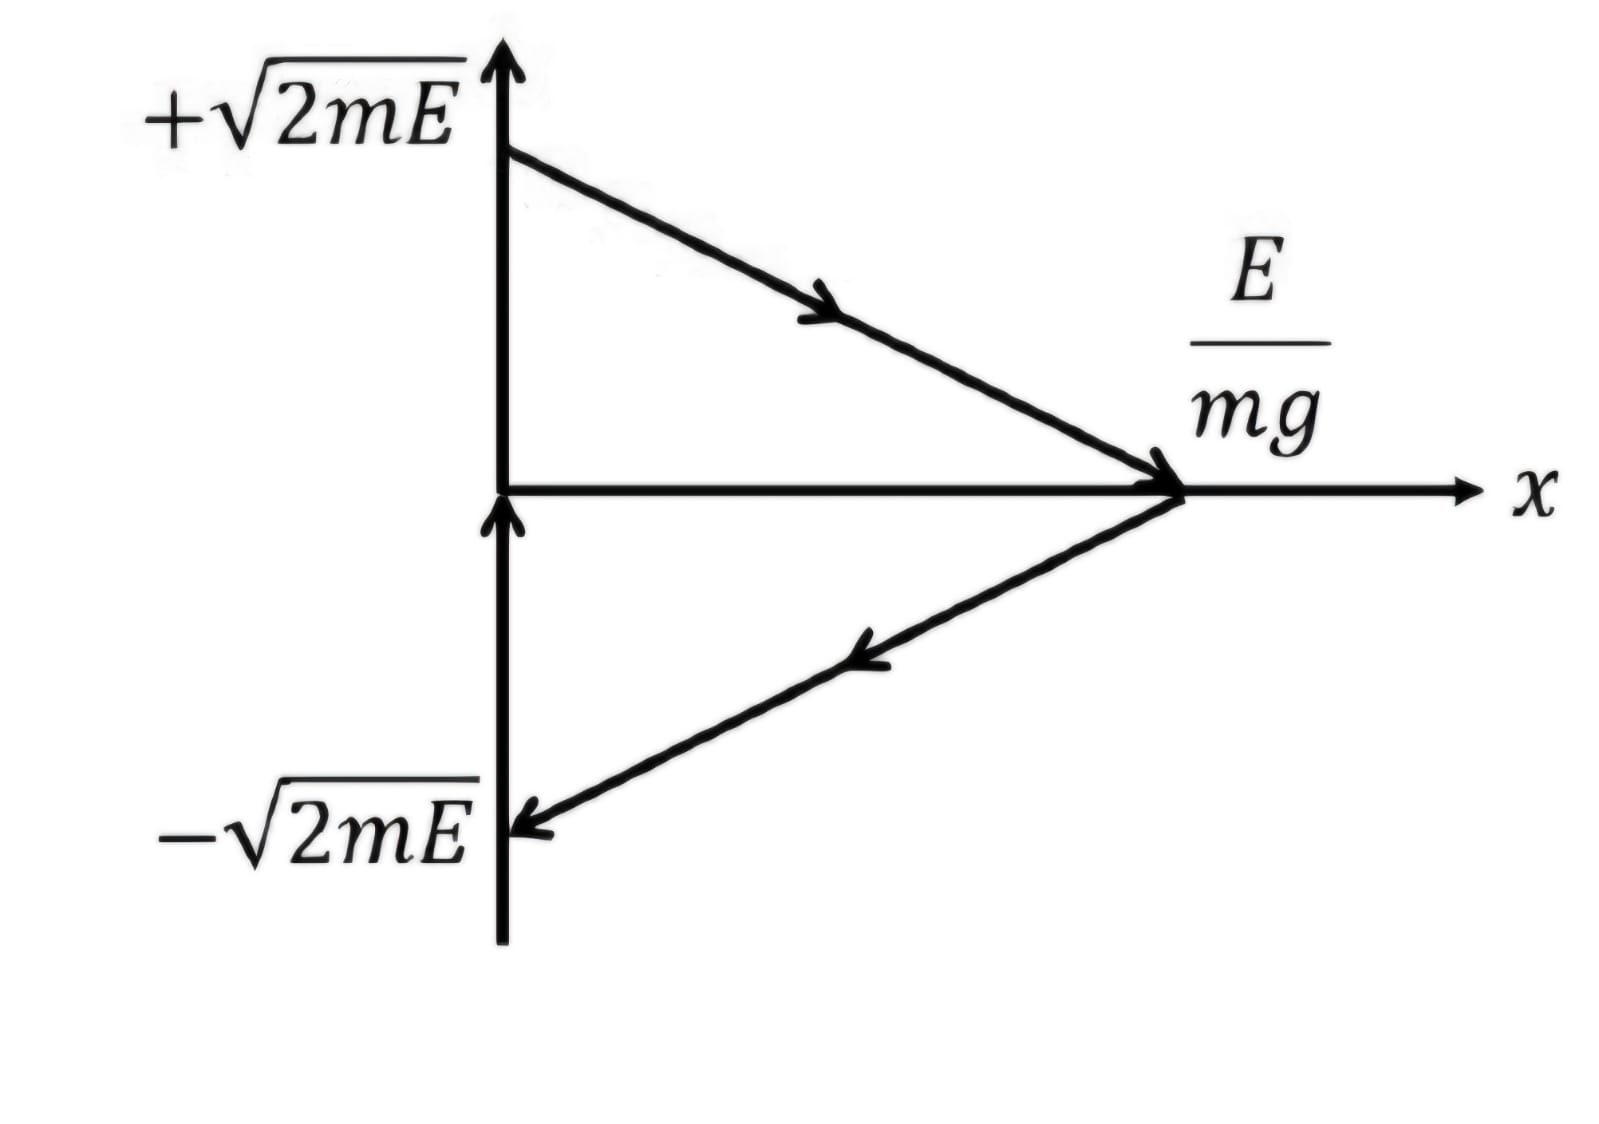
\includegraphics[width=0.35\textwidth]{fig9.jpeg} \hfill
    \item 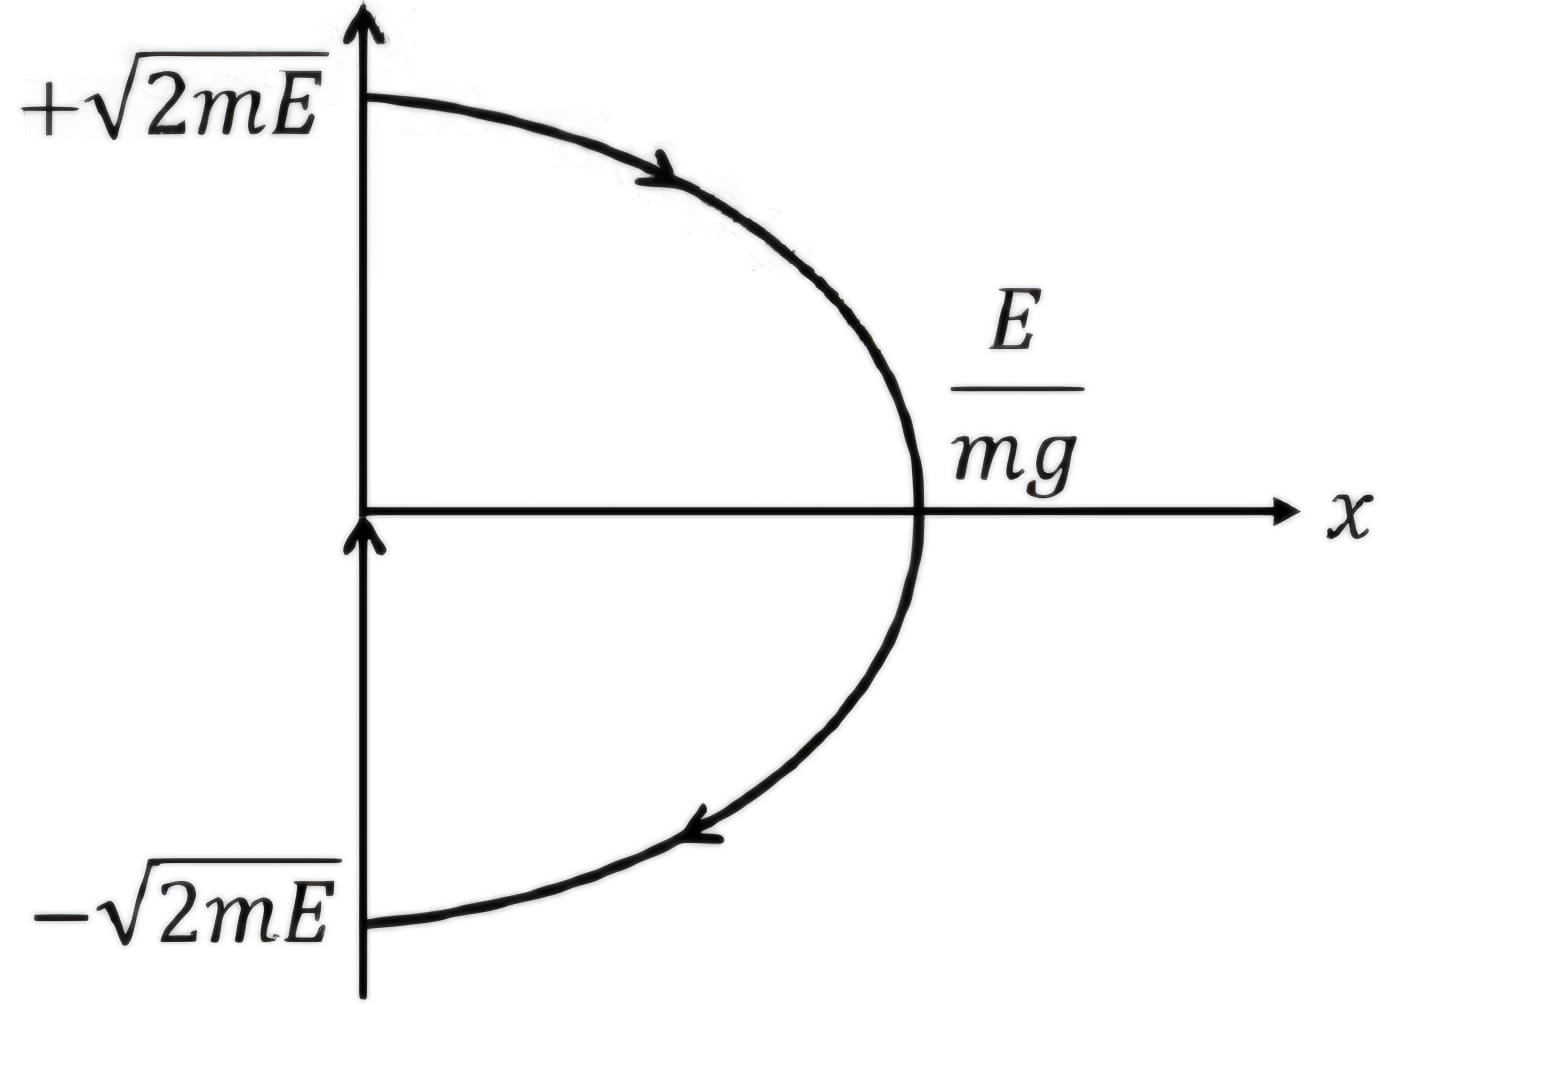
\includegraphics[width=0.35\textwidth]{fig10.jpeg} \hfill
    \item 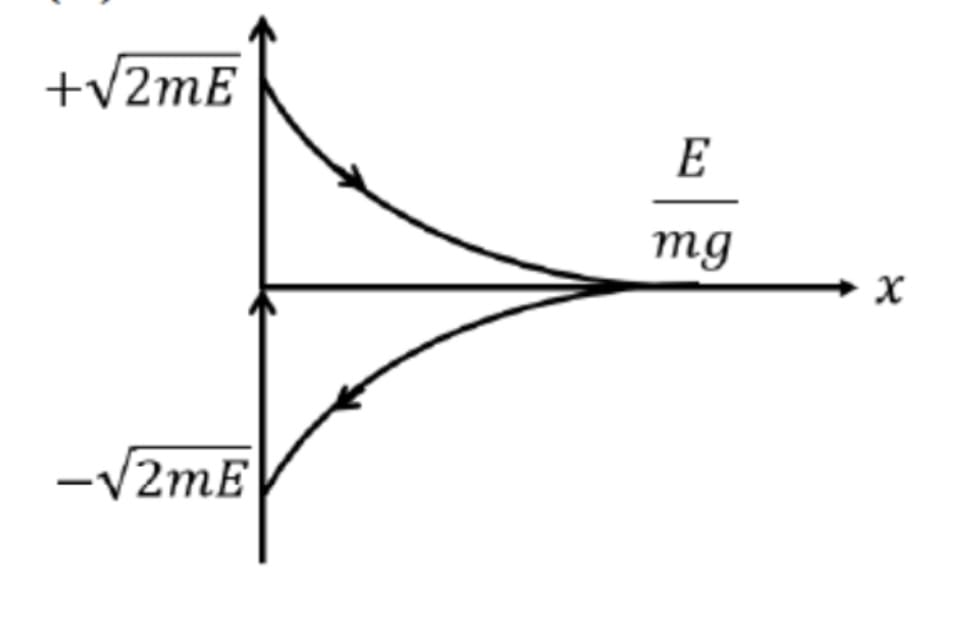
\includegraphics[width=0.35\textwidth]{fig11.jpeg} \hfill
    \item 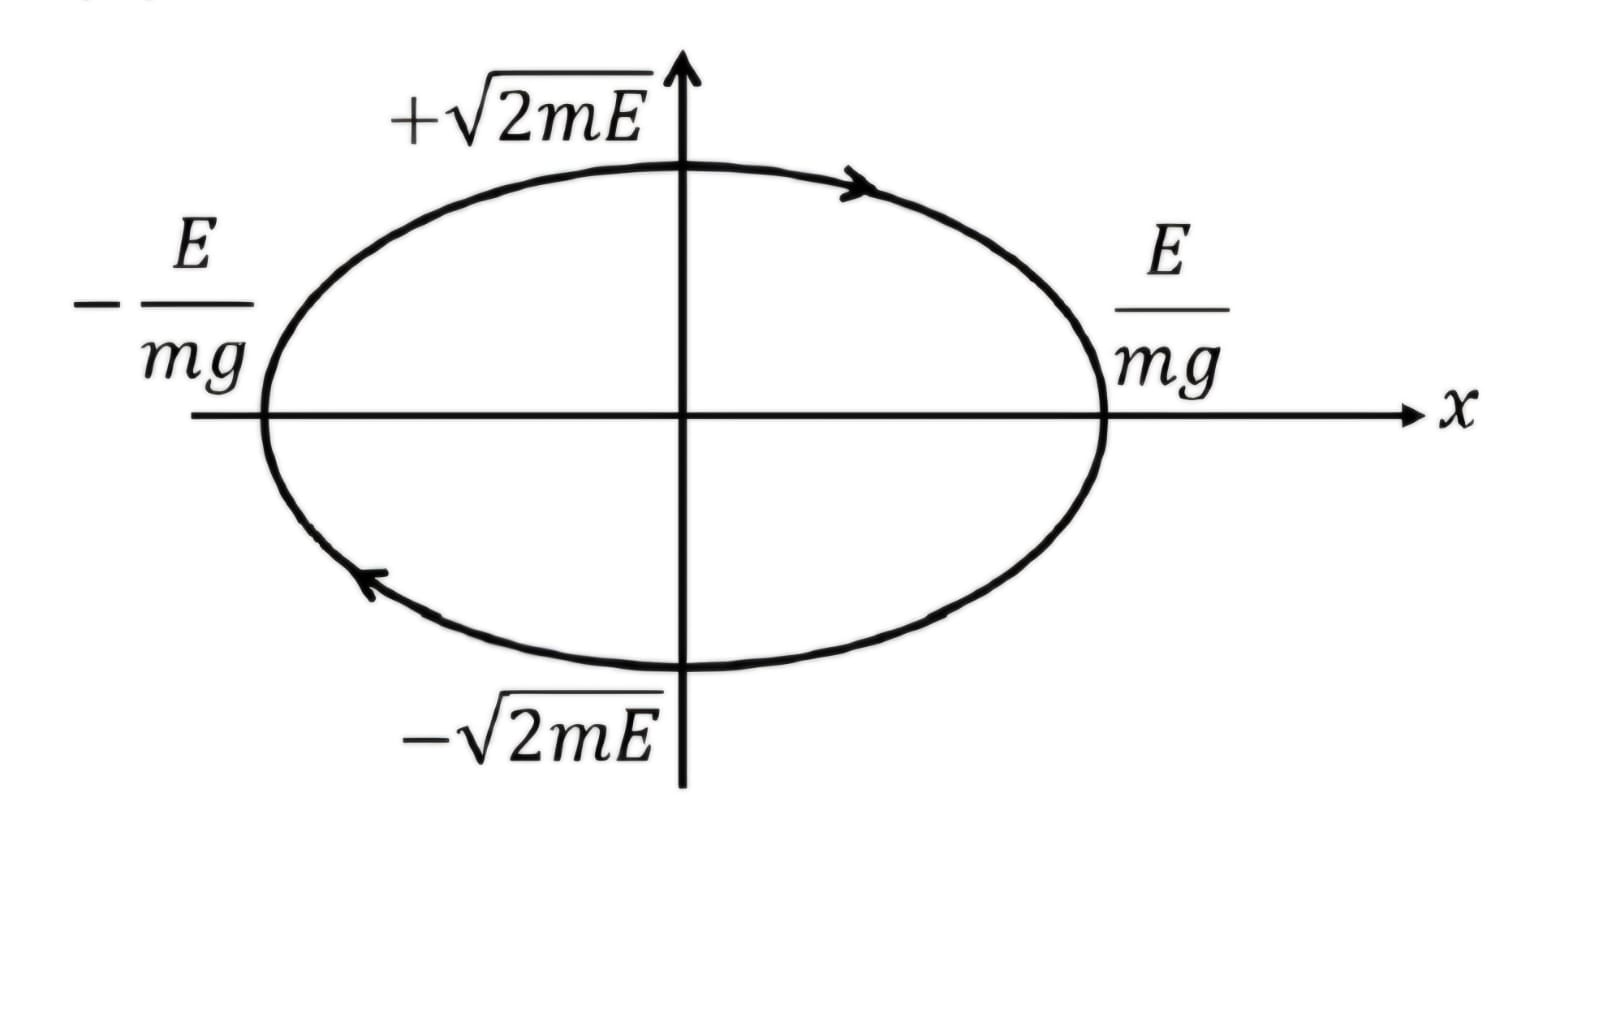
\includegraphics[width=0.4\textwidth]{fig12.jpeg} \hfill
\end{enumerate}
\end{multicols}

\newpage

\item An infinitely long wire parallel to the $x$-axis is kept at $z=d$ and carries a current $I$ in the positive $x$-direction above a superconductor filling the region $z \leq 0$ (see figure). The magnetic field $\vec{B}$ inside the superconductor is zero so that the field just outside the superconductor is parallel to its surface. The magnetic field due to this configuration at a point $(x, y, z>0)$ is

\begin{figure}[ht!]
    \centering
    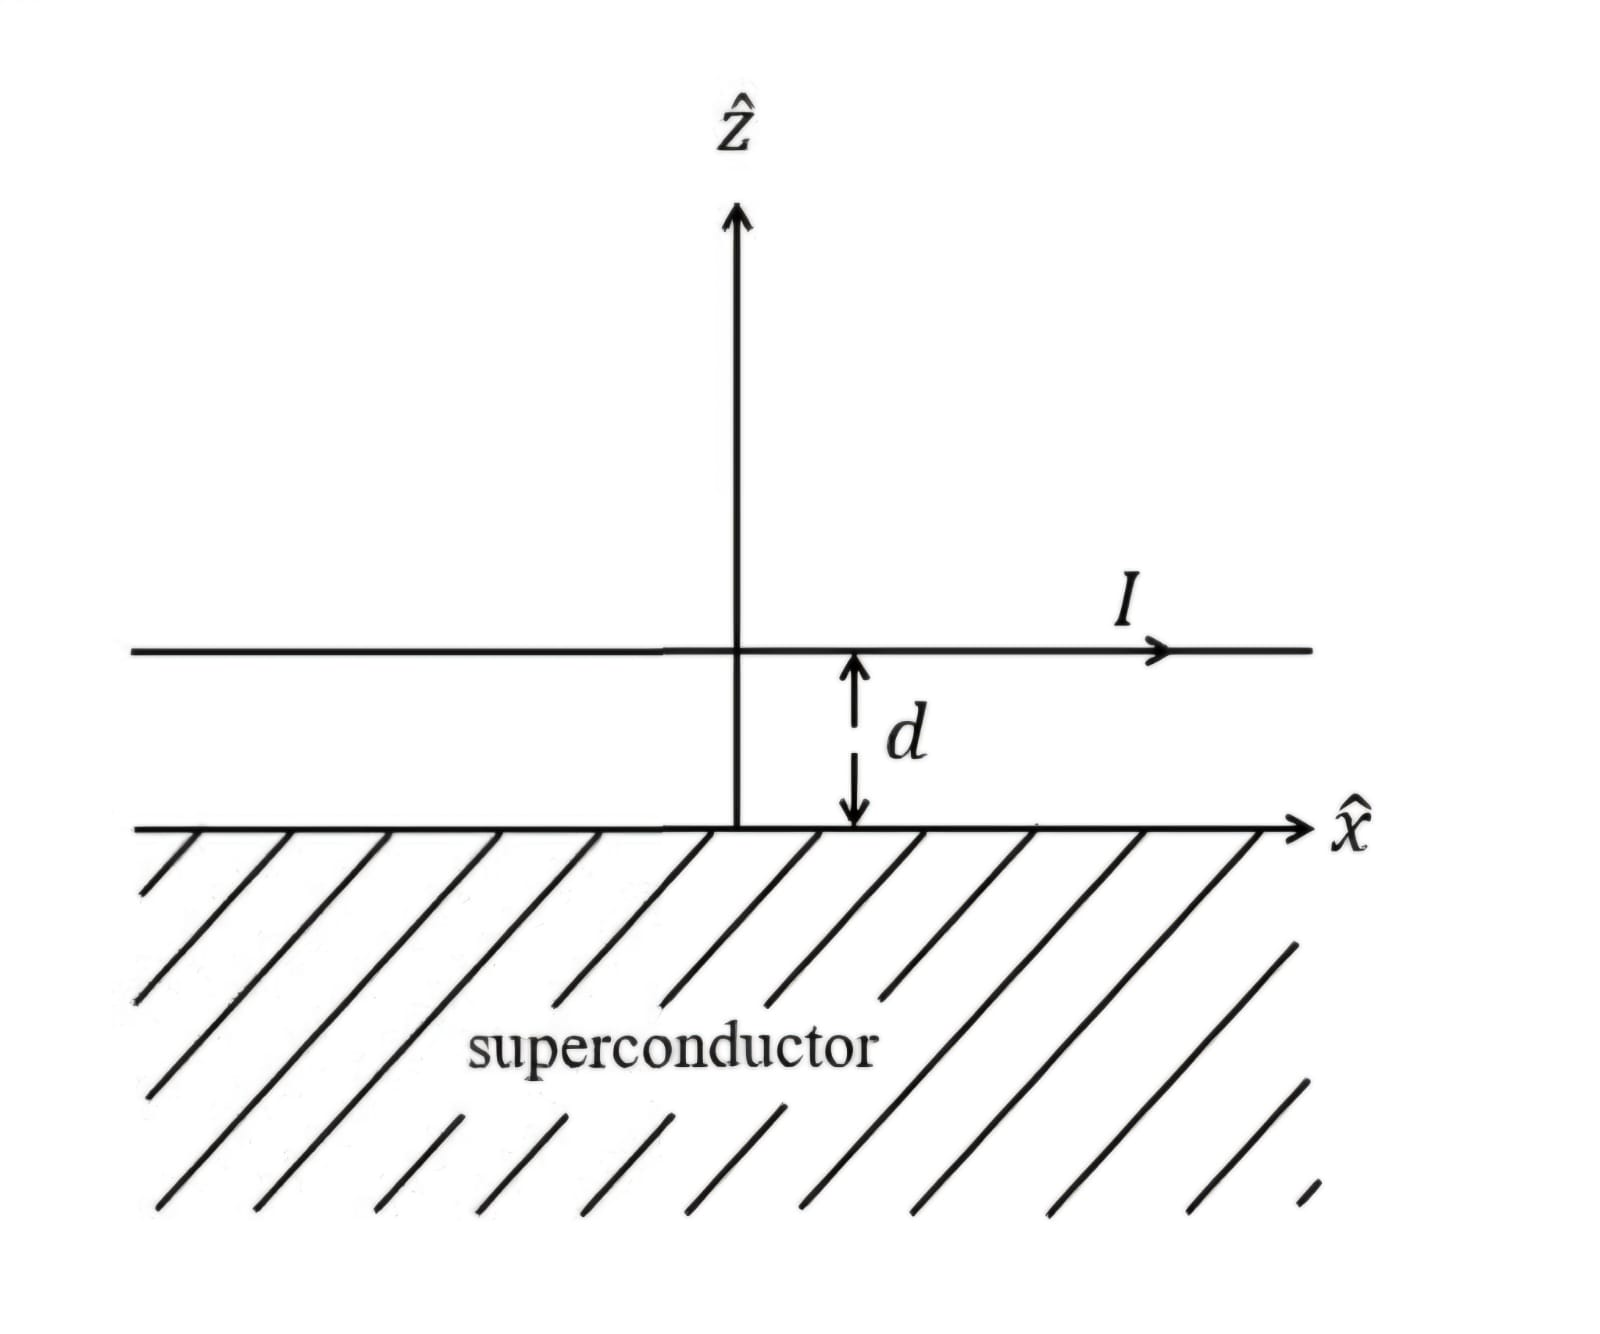
\includegraphics[width=0.5\textwidth]{fig13.jpeg}
    \caption{}
    \label{fig:fig13.jpeg}
\end{figure}

\hfill{\brak{\text{GATE IN 2019}}}



    \begin{enumerate}
        \item $\dfrac{\mu_{0} I}{2\pi} \dfrac{-(z-d)\,\hat{i}+y\,\hat{k}}{y^{2}+(z-d)^{2}}$
        \item $\dfrac{\mu_{0} I}{2\pi} \left[\dfrac{-(z-d)\,\hat{i}+y\,\hat{k}}{y^{2}+(z-d)^{2}} + \dfrac{(z+d)\,\hat{i}-y\,\hat{k}}{y^{2}+(z+d)^{2}}\right]$
        \item $\dfrac{\mu_{0} I}{2\pi} \left[\dfrac{-(z-d)\,\hat{i}+y\,\hat{k}}{y^{2}+(z-d)^{2}} - \dfrac{(z+d)\,\hat{i}-y\,\hat{k}}{y^{2}+(z+d)^{2}}\right]$d
        \item $\dfrac{\mu_{0} I}{2\pi} \left[\dfrac{y\,\hat{j}+(z-d)\,\hat{k}}{y^{2}+(z-d)^{2}} + \dfrac{y\,\hat{j}-(z+d)\,\hat{k}}{y^{2}+(z+d)^{2}}\right]$
    \end{enumerate}
    
    \item The vector potential inside a long solenoid, with turns per unit length $n$ and carrying current $I$, written in cylindrical coordinates is   \[\vec{A}(s,\phi,z) = \frac{\mu_{0} n I}{2}\,s\,\hat{\phi}. \]. If the term\[\frac{\mu_{0} n I}{c^{2}}\,s \,(\alpha \cos\phi\,\hat{\phi} + \beta \sin\phi\,\hat{s}), \] 
   
    where $\alpha \neq 0$ and $\beta \neq 0$, is added to $\vec{A}(s,\phi,z)$, the magnetic field remains the same if

    \hfill{\brak{\text{GATE IN 2019}}}

    \begin{multicols}{4}
    \begin{enumerate}
        \item $\alpha = \beta$
        \item $\alpha = -\beta$
        \item $\alpha = 2\beta$
        \item $\alpha = \dfrac{\beta}{2}$
    \end{enumerate}
    \end{multicols}


\item Low energy collision (s-wave scattering) of pion ($\pi^{-}$) with deuteron ($d$) results in the production of two protons 
    \[
    \pi^{-} + d \;\;\rightarrow\;\; p + p.
    \]
    The relative orbital angular momentum (in units of $\hbar$) of the resulting two-proton system for this reaction is

    \hfill{\brak{\text{GATE IN 2019}}}
    
    \begin{multicols}{4}
    \begin{enumerate}
        \item 0
        \item 1
        \item 2
        \item 3
    \end{enumerate}
    \end{multicols}

    \item Consider the Hamiltonian 
    \[
    H(q,p) = \frac{\alpha p^{2} q^{4}}{2} + \frac{\beta}{q^{2}},
    \]
    where $\alpha$ and $\beta$ are parameters with appropriate dimensions, and $q, p$ are generalized coordinate and momentum, respectively. The corresponding Lagrangian $L(q,\dot{q})$ is

    \hfill{\brak{\text{GATE IN 2019}}}
    
    \begin{multicols}{4}
    \begin{enumerate}
        \item $\tfrac{1}{2}\alpha \dot{q}^{2} q^{4} - \dfrac{\beta}{q^{2}}$
        \item $\dfrac{2}{\alpha}\,\dfrac{q^{2}}{q^{4}} + \dfrac{\beta}{q^{2}}$
        \item $\alpha \dot{q}^{2} q^{4} + \dfrac{\beta}{q^{2}}$
        \item $-\tfrac{1}{2}\alpha \dot{q}^{2} q^{4} + \dfrac{\beta}{q^{2}}$
    \end{enumerate}
    \end{multicols}

    \item For a given load resistance $R_{L}=4.7~\Omega$, the power transfer efficiencies 
    \[
    \eta = \frac{P_{\text{load}}}{P_{\text{total}}}
    \]
    of a DC voltage source and a DC current source with internal resistances $R_{1}$ and $R_{2}$ respectively, are equal. The product $R_{1}R_{2}$, in units of $\Omega$ (rounded off to one decimal place), is \\\\\_.

    \hfill{\brak{\text{GATE IN 2019}}}

    \item The ground state electronic configuration of the rare-earth ion $Nd^{3+}$ is 
    \[
    [Pd]\,4f^{3}5s^{2}5p^{6}.
    \]
    Assuming $LS$ coupling, the Landé $g$-factor of this ion is $\tfrac{8}{11}$. The effective magnetic moment in units of Bohr magneton $\mu_{B}$ (rounded off to two decimal places) is \\\\\_.

    \hfill{\brak{\text{GATE IN 2019}}}

    \item A projectile of mass $1~\text{kg}$ is launched at an angle of $30^{\circ}$ from the horizontal at $t=0$ and takes time $T$ before hitting the ground. If its initial speed is $10~\text{m/s}$, the value of the action integral for the entire flight in units of $\text{kg}\,\text{m}^{2}\,\text{s}^{-1}$ (rounded off to one decimal place) is \\\\\_. 

    \hfill{\brak{\text{GATE IN 2019}}}
    \[
    \text{Take } g = 10~\text{m/s}^{2}.
    \]

    \item Let $\theta$ be a variable in the range $-\pi \leq \theta < \pi$. Consider the function
    \[
    \psi(\theta) = 
    \begin{cases}
        1, & -\tfrac{\pi}{2} \leq \theta < \tfrac{\pi}{2}, \\[6pt]
        0, & \text{otherwise}.
    \end{cases}
    \]
    If its Fourier-series is written as
    \[
    \psi(\theta) = \sum_{m=-\infty}^{\infty} C_{m} e^{-im\theta},
    \]
    then the value of $\lvert C_{3} \rvert^{2}$ (rounded off to three decimal places) is \\\\\_.

    \hfill{\brak{\text{GATE IN 2019}}}

    \item Two space ships A and B, each of the same rest length L, are moving in the same direction with speeds $\frac{4C}{5}$ and $\frac{3C}{5}$ , respectively. As mentioned by B, the time taken by A to completely overtake B in units of $\frac{L}{c}$is

    \begin{figure}[ht!]
    \centering
    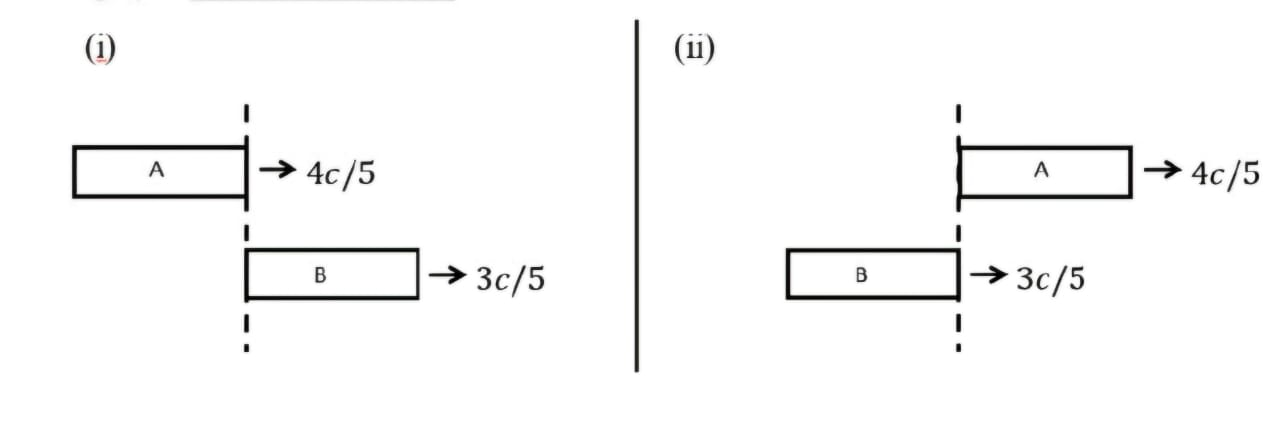
\includegraphics[width=1\textwidth]{fig14.jpeg}
    \caption{}
    \label{fig:fig14.jpeg}
    \end{figure}

    \hfill{\brak{\text{GATE IN 2019}}}

    \item A radioactive element $X$ has a half-life of $30$ hours. It decays via $\alpha$, $\beta$ and $\gamma$ emissions with the branching ratio for $\beta$ decay being $0.75$. The partial half-life for $\beta$ decay in units of hours is

    \hfill{\brak{\text{GATE IN 2019}}}

   \item In a thermally insulated container, $0.01\ \mathrm{kg}$ of ice at $273\ \mathrm{K}$ is mixed with $0.1\ \mathrm{kg}$ of water at $300\ \mathrm{K}$. Neglecting the specific heat of the container, the change in the entropy of the system in $\mathrm{J/K}$ on attaining thermal equilibrium (rounded off to two decimal places) is  

  

  (Specific heat of water is $4.2\ \mathrm{kJ\,kg^{-1}\,K^{-1}}$ and the latent heat of ice is $335\ \mathrm{kJ\,kg^{-1}}$.)

   \hfill{\brak{\text{GATE IN 2019}}}

   \newpage

   \item Consider a system of three charges as shown in the figure below:

   \begin{figure}[ht!]
    \centering
    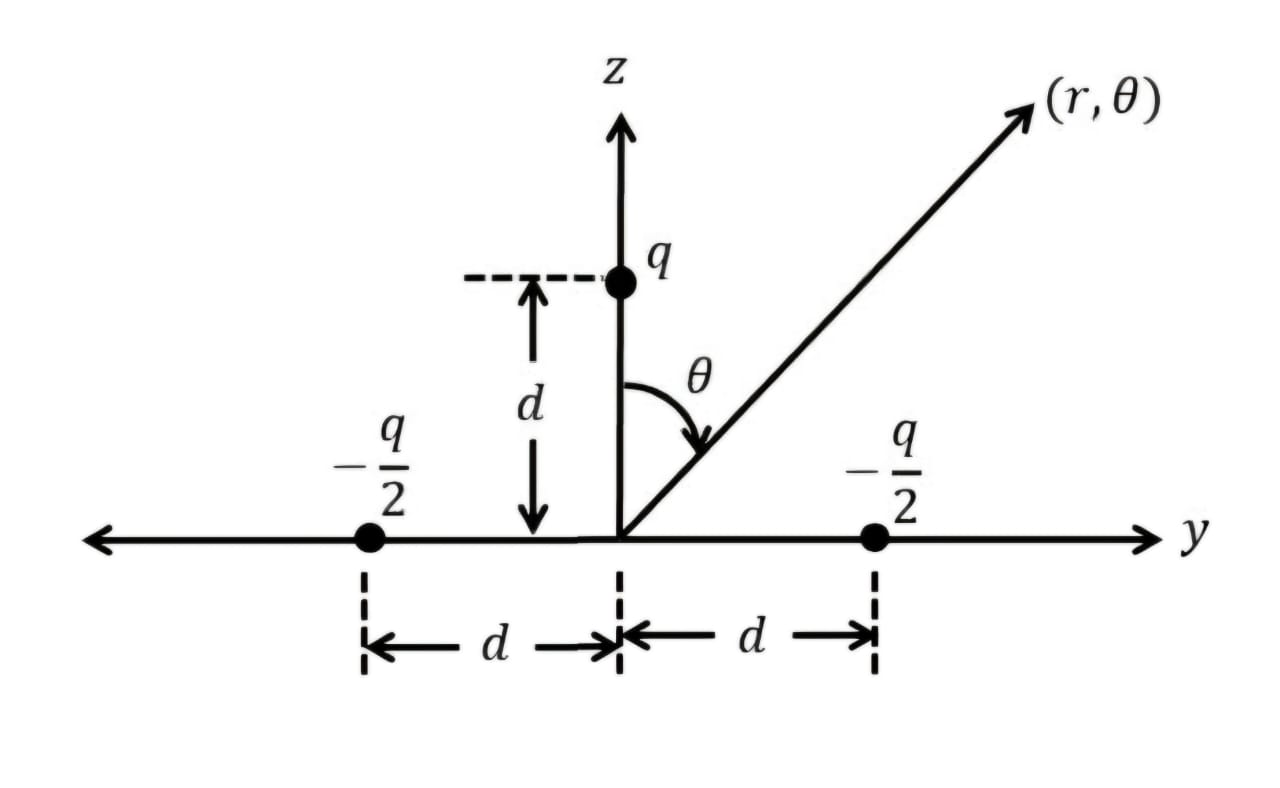
\includegraphics[width=0.5\textwidth]{fig15.jpeg}
    \caption{}
    \label{fig:fig15.jpeg}
    \end{figure}

    For $r = 10\ \mathrm{m}$, $\theta = 60^\circ$, $q = 10^{-6}\ \mathrm{Coulomb}$, and $d = 10^{-3}\ \mathrm{m}$, the electric dipole potential (in volts, rounded off to decimal places) at a point $(r,0)$ is  

  [Use: $\tfrac{1}{4\pi\epsilon_{0}} = 9 \times 10^9\ \mathrm{N\,m^2/C^2}$]

  \hfill{\brak{\text{GATE IN 2019}}}
  

  \item Consider two systems A and B each having two distinguishable particles. In both the systems, each particle can exist in states with energies $0,1,2,3$ units with equal probability. The total energy of the combined system is $5$ units. Assuming that the system A has energy $3$ units and the system B has energy $2$ units, the entropy of the combined system is $\ln \lambda$. The value of $\lambda$ is $k_B$.

  \hfill{\brak{\text{GATE IN 2019}}}

  \item Electrons with spin in the $z$-direction ($\uparrow_z$) are passed through a Stern-Gerlach (SG) set up with the magnetic field at $\theta = 60^\circ$ from $z$. The fraction of electrons that will emerge with their spin parallel to the magnetic field in the SG set up (rounded off to two decimal places) is  

    \begin{align*}
     \sigma_{y} = \myvec{0 & -i \\i & 0}
    ,\quad
    \sigma_{x} =  \myvec{ 0 & 1 \\  1 & 0}
    ,\quad
    \sigma_{z} = \myvec{ 1 & 0 \\ 0 & -1}
    \end{align*}
  
  

  \hfill{\brak{\text{GATE IN 2019}}}

  \item The Hamiltonian of a system is 
  \begin{align*}
   H = \myvec{ 1 & \epsilon \\ \epsilon & -1}
    , \qquad \epsilon \ll 1
  \end{align*}
  
  The fourth-order contribution to the ground state energy of $H$ is $\gamma \epsilon^4$. The value of $\gamma$ (rounded off to three decimal places) is

  \hfill{\brak{\text{GATE IN 2019}}}

  \newpage

  \item Two events, one on the Earth and the other one on the Sun, occur simultaneously in the Earth's frame. The time difference between the two events as seen by an observer in a spaceship moving with velocity $0.5c$ in the Earth's frame along the line joining the Earth to the Sun is $\Delta t$, where $c$ is the speed of light.  

  Given that light travels from the Sun to the Earth in $8.3$ minutes in the Earth's frame, the value of $\Delta t$ in minutes (rounded off to two decimal places) is  

  \hfill{\brak{\text{GATE IN 2019}}}

  
  \item In a certain two-dimensional lattice, the energy dispersion of the electrons is  
  \[
    \varepsilon(\vec{k}) = -2t\cos(k_x a) + 2\cos(k_y a)\cos(k_x a),
  \]
  where $\vec{k} = (k_x, k_y)$ denotes the wave vector, $a$ is the lattice constant, and $t$ is a constant in units of eV.  

  In this lattice the effective mass tensor $m^*_{ij}$ of electrons calculated at the center of the Brillouin zone is

  \hfill{\brak{\text{GATE IN 2019}}}
 

    
\end{enumerate}
\end{document}
